% Leveraging I/O Configurability of Amazon EC2 Cloud
% % @author Mingliang Liu % @date 2011-6-14 

\documentclass{beamer}
\usetheme{progressbar}
\progressbaroptions{headline=none, frametitle=picture-section,
                    titlepage=picture, imagename=thu}
\usepackage{times}
\usepackage{graphicx}
\usepackage{color}
\usepackage{fancybox}
\usepackage{booktabs}
\usepackage{hyperref}
\usepackage{wasysym}

\begin{document}

\title{One Optimized I/O Configuration per HPC Application}
\subtitle{Leveraging I/O Configurability of Amazon EC2 Cloud}
\author{
    \parbox[t]{5.5cm}{
        \hfill Mingliang Liu, Jidong Zhai, Yan Zhai \hfill
        \\\hbox{}
        \hfill{\tiny Tsinghua University}\hfill\hbox{}
    }\\
    \vspace{.5cm}
    \parbox[t]{3.5cm}{
        \hfill Xiaosong Ma~ ~ ~ ~ ~ \hfill
        \\\hbox{}
        \hfill {\tiny {North Carolina State University}}\hfill \hbox{}
        \\\hbox{}
        \hfill {\tiny Oak Ridge National Laboratory}\hfill \hbox{}
    }
    \parbox[t]{2.5cm}{
        \hfill Wenguang Chen \hfill
        \\\hbox{}
        \hfill {\tiny {Tsinghua University}}\hfill \hbox{}
    }
}
\date{APSys 2011, July 12}

%%%%%%%%%%%%%%%%%%%%%%%%  Preamble %%%%%%%%%%%%%%%%%%%%%%%%%
\begin{frame}
    \titlepage
\end{frame}

%%%%%%%%%%%%%%%%%%%%%%% Introduction %%%%%%%%%%%%%%%%%%%%%%%%
\section{Introduction}
\begin{frame}{Outline}
    \tableofcontents[current]
\end{frame}

\begin{frame}{Background}
    \begin{itemize}
        \item I/O becomes the bottleneck for many HPC applications
            \begin{itemize}
                \item Intensive I/O operations and concurrency
                \item One-size-fits-all I/O configuration
            \end{itemize}
        \item There is a trend to migrate the HPC applications from traditional
            platforms to cloud
        \item Cloud provides tremendous flexibility in configuring I/O system
            \begin{itemize}
                \item Fully controlled virtual machines
                \item Easily deployed user scripts
                \item Multiple types of low-level devices
                \item Online device acquisition and migration
            \end{itemize}
    \end{itemize}
\end{frame}

\begin{frame}{Motivation}
    \begin{block}{The Problem}
        Can we employ I/O configurability of cloud for HPC apps?
    \end{block}
    \pause
    {\huge\smiley} Configurability lies in:
    \begin{itemize}
            \item Set up the specific file system at start up
            \item Explore different types of low-level devices
            \item Tune the file system inherent parameters
    \end{itemize}
    \pause
    {\huge\frownie} Challenges:
    \begin{itemize}
        \item The feasibility is highly workload-dependent
        \item Tradeoff between efficiency vs. cost-effectiveness
    \end{itemize}
\end{frame}

\begin{frame}{Amazon EC2 CCI}
    \begin{exampleblock}{CCI: Cluster Computing Instance}
        Amazon's solution to HPC in Cloud
    \end{exampleblock}
    \begin{itemize}
        \item Quad-core Intel Xeon X5570 CPU, with 23GB memory
        \item Interconnected by 10 Gigabit Ethernet
        \item Amazon Linux AMI, RedHat family OS with Intel MPI
        \item local block storage (Ephemeral) with 2*800 GB
        \item Elastic Block Store (EBS), attached as block storage devices
        \item Simple Storage Service (S3), key-value based object storage
    \end{itemize}
\end{frame}

%%%%%%%%%%%%%%%%%%%%%%% Storage System Options %%%%%%%%%%%%%%%%%%%%%%
\section{Storage System Options in the Amazon EC2 CCI}
\begin{frame}{Outline}
    \tableofcontents[current]
\end{frame}

\begin{frame}{File System Selection}
    \begin{itemize}
        \item Different I/O access pattern and concurrency require different kinds of
            file system\\
            - shared vs. parallel
        \item NFS is enough for low I/O demands, simple to deploy
        \item A parallel file system (eg. PVFS, Lustre) can be employed to
            \begin{itemize} 
                \item support large and shared file writes
                \item scale up well
            \end{itemize}
    \end{itemize}
    \pause
    \begin{exampleblock}{Easy to choose and setup}
        118 LOC bash for NFS, and 173 LOC bash for PVFS
    \end{exampleblock}
\end{frame}

\begin{frame}{Device Selection Considerations}
    Devices differ in levels of abstraction and access interfaces.
    \begin{tabular}{p{2.0cm}|p{5.0cm}|p{3.0cm}}
        \toprule
        \textbf{Storage} & \textbf{Pros.} & \textbf{Cons.} \\
        \midrule
        \textbf{S3}      &
            off-shelf, designed for Internet and database apps &
            no POSIX \\
        \midrule
        \textbf{Ephemeral} &
            Free & non-persistent, only two disks\\
        \midrule
        \textbf{EBS} &
            - persistent beyond instances - more disks available &
            Charged \\
        \bottomrule
    \end{tabular}
    \vspace{.3cm}
    \pause
    \begin{block}{}
        The choice depends on the needs of individual \emph{applications}
    \end{block}
\end{frame}

\begin{frame}{File System Internal Parameters}
    \begin{tabular}{p{3.7cm}|p{6.3cm}}
        \toprule
        \textbf{Options} & \textbf{Description} \\
        \midrule
        \textit{Sync mode} &
            NFS \texttt{sync} vs \texttt{async} write modes \\
        \textit{Device number} &
            Combining multiple disks into a software RAID0 \\
        \textit{I/O server number} &
            NFS single-server bottleneck, PVFS can employ many I/O servers \\
        \textit{Meta-data distribution} &
            PVFS can distribute metadata to multiple servers \\
        \textit{I/O Server Placement} &
            Part-time vs. dedicated I/O servers \\
        \textit{Data Striping} & 
            striping factor, unit size\\
        \bottomrule
    \end{tabular}
    \vspace{.2cm}
    \pause
    \begin{block}{Again}
        The choice depends on the needs of individual \emph{applications}
    \end{block}
\end{frame}

\begin{frame}{Dedicated NFS, Ephemeral Disks}
    \begin{center}
        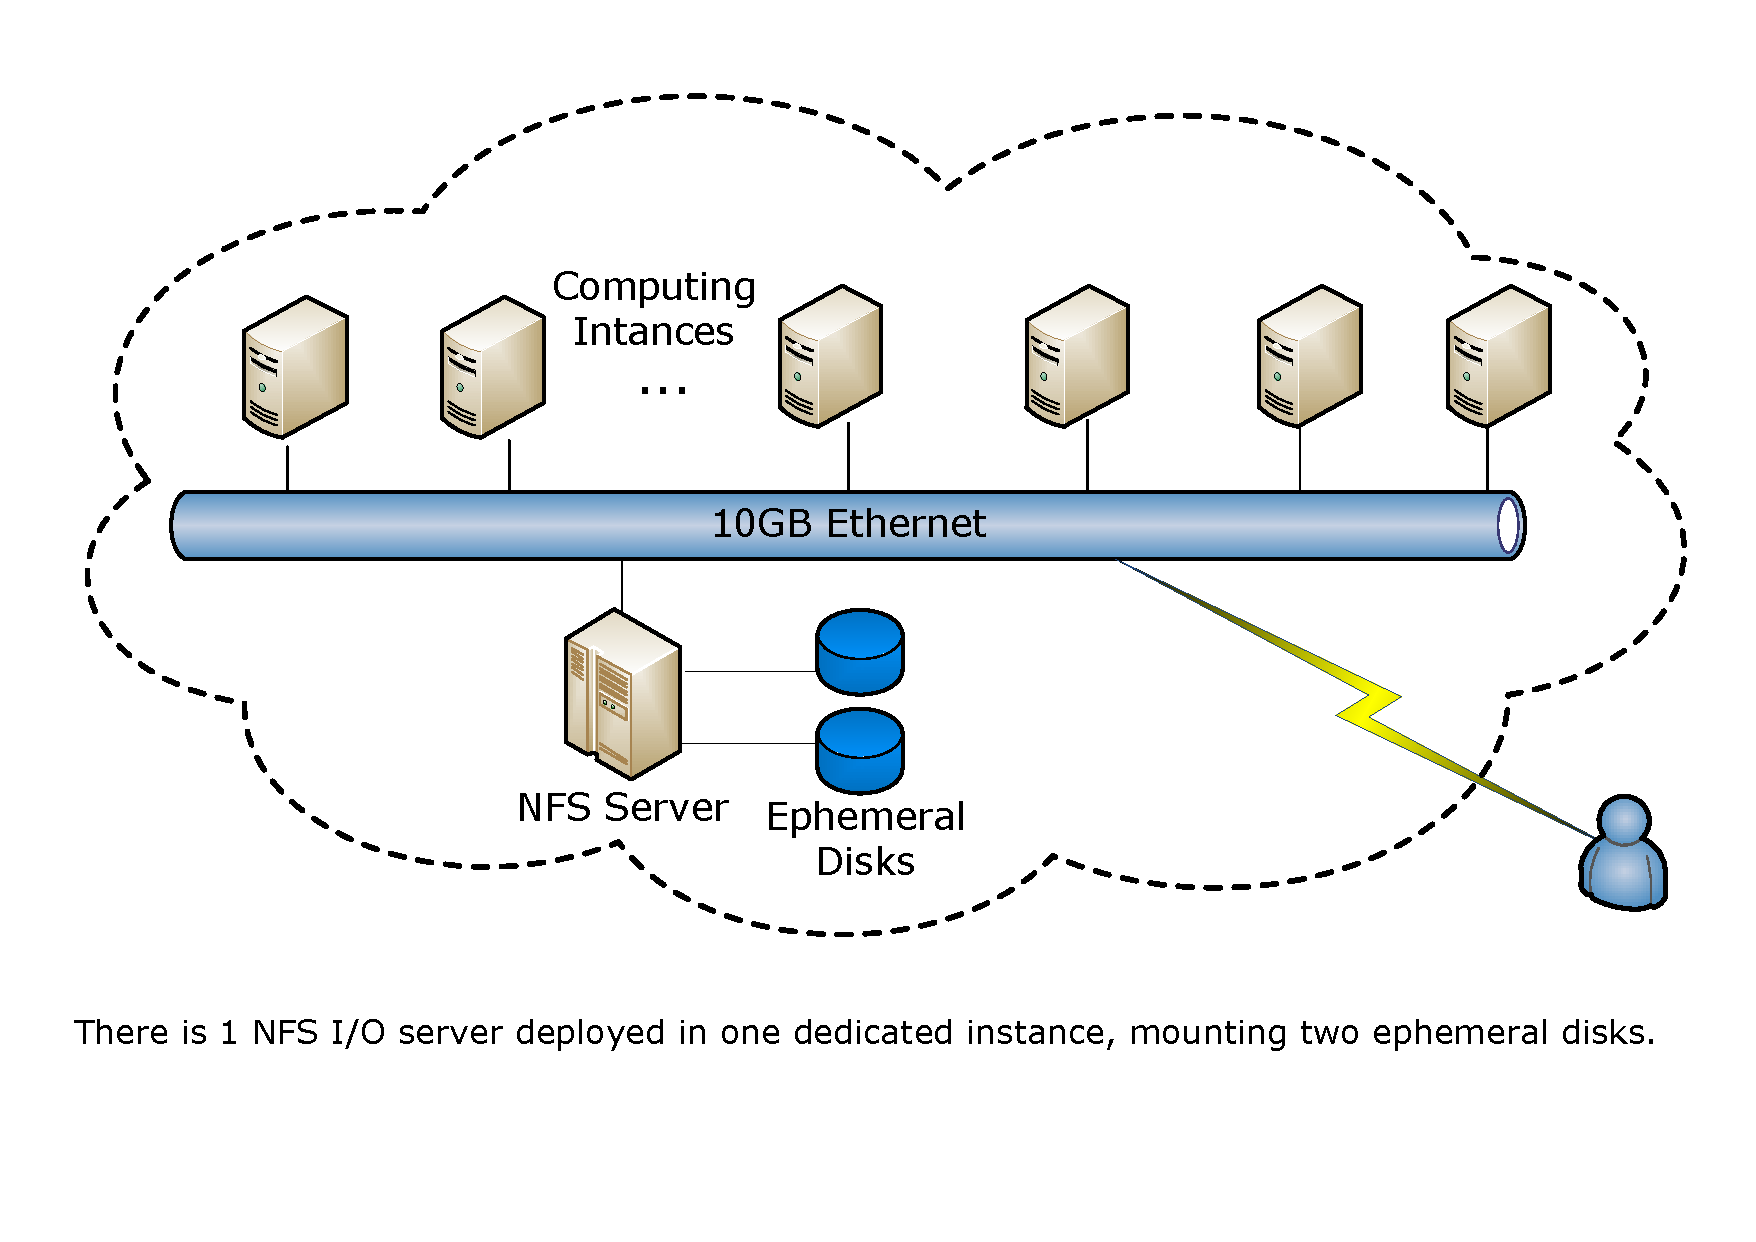
\includegraphics[width=\textwidth]{figures/visio/nfs-ephemeral.pdf}
    \end{center}
\end{frame}

\begin{frame}{Parttime NFS Mounting Ephemeral}
    \begin{center}
        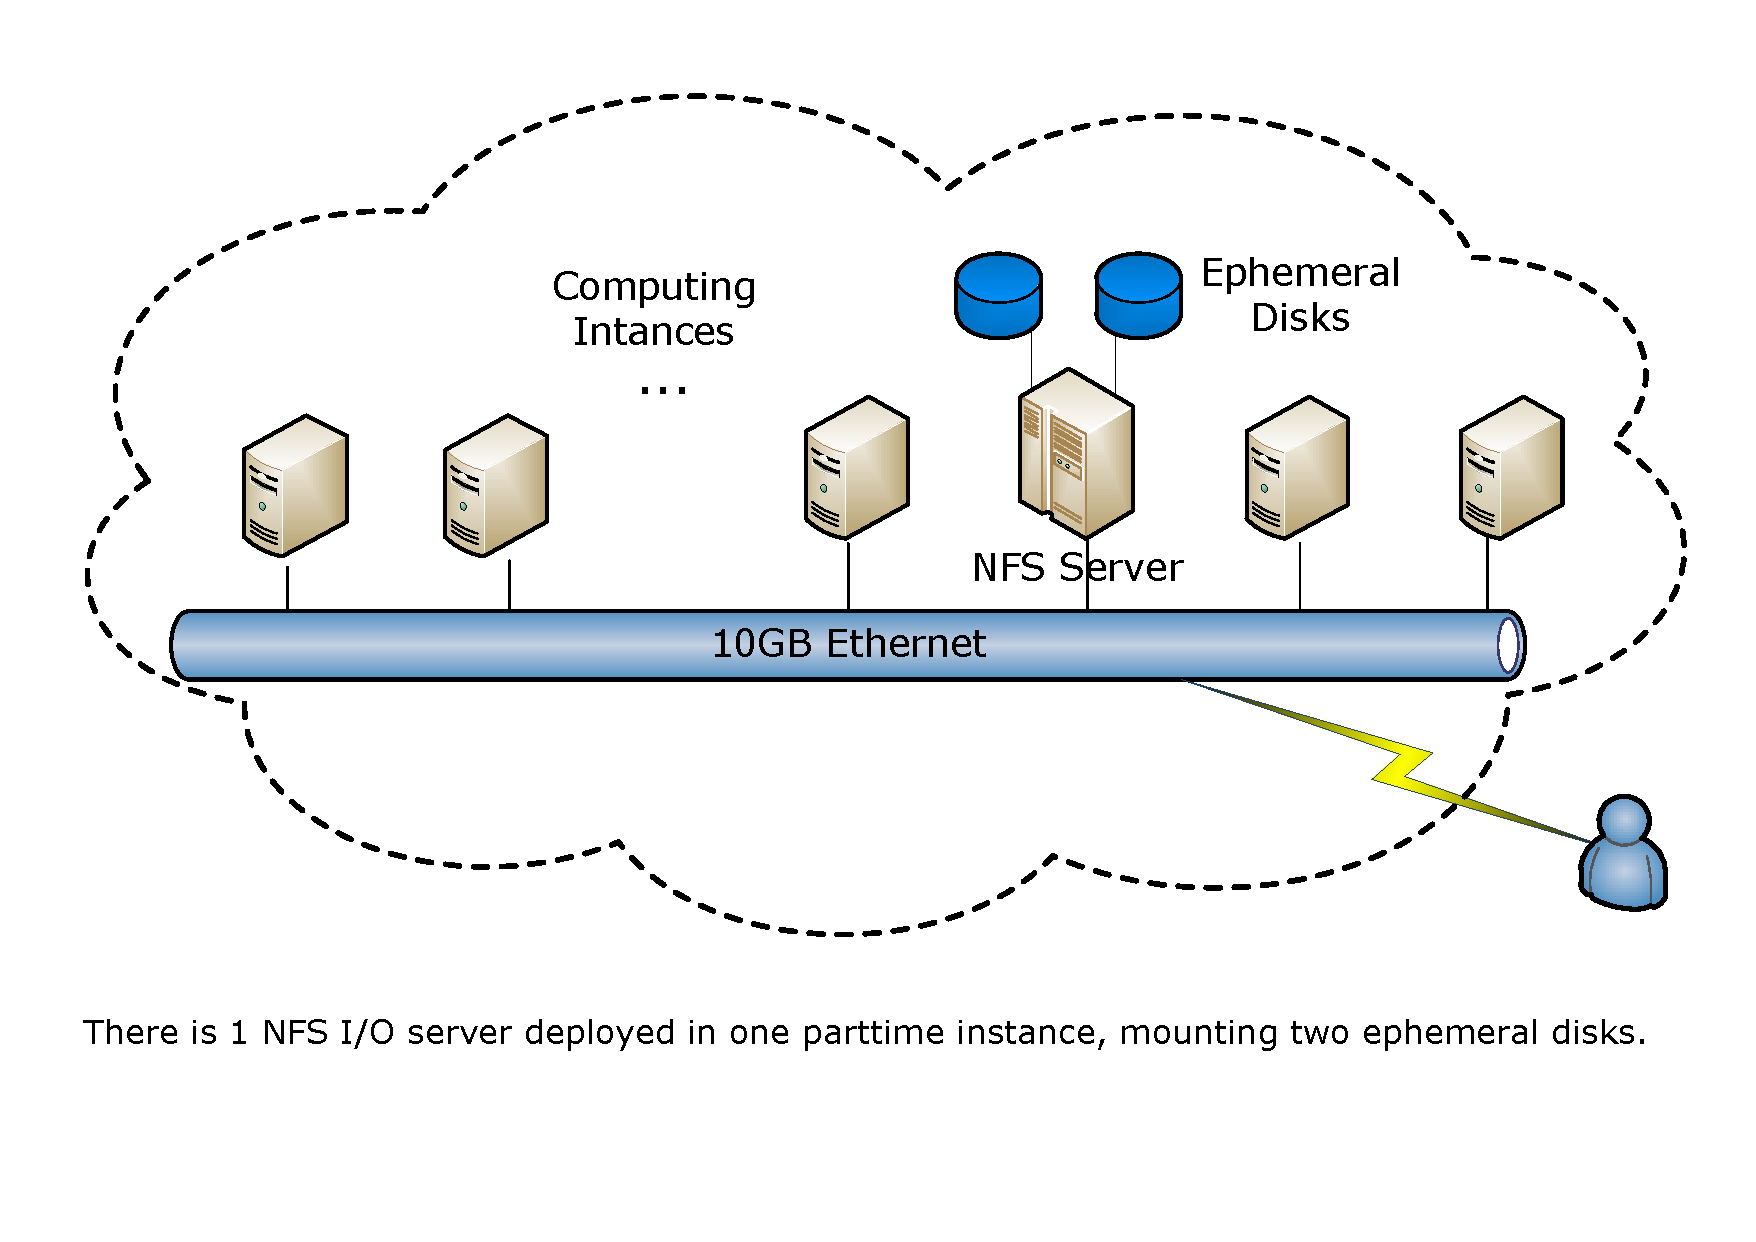
\includegraphics[width=\textwidth]{figures/visio/nfs-ephemeral-part.pdf}
    \end{center}
\end{frame}

\begin{frame}{Dedicated NFS Mounting EBS Disks}
    \begin{center}
        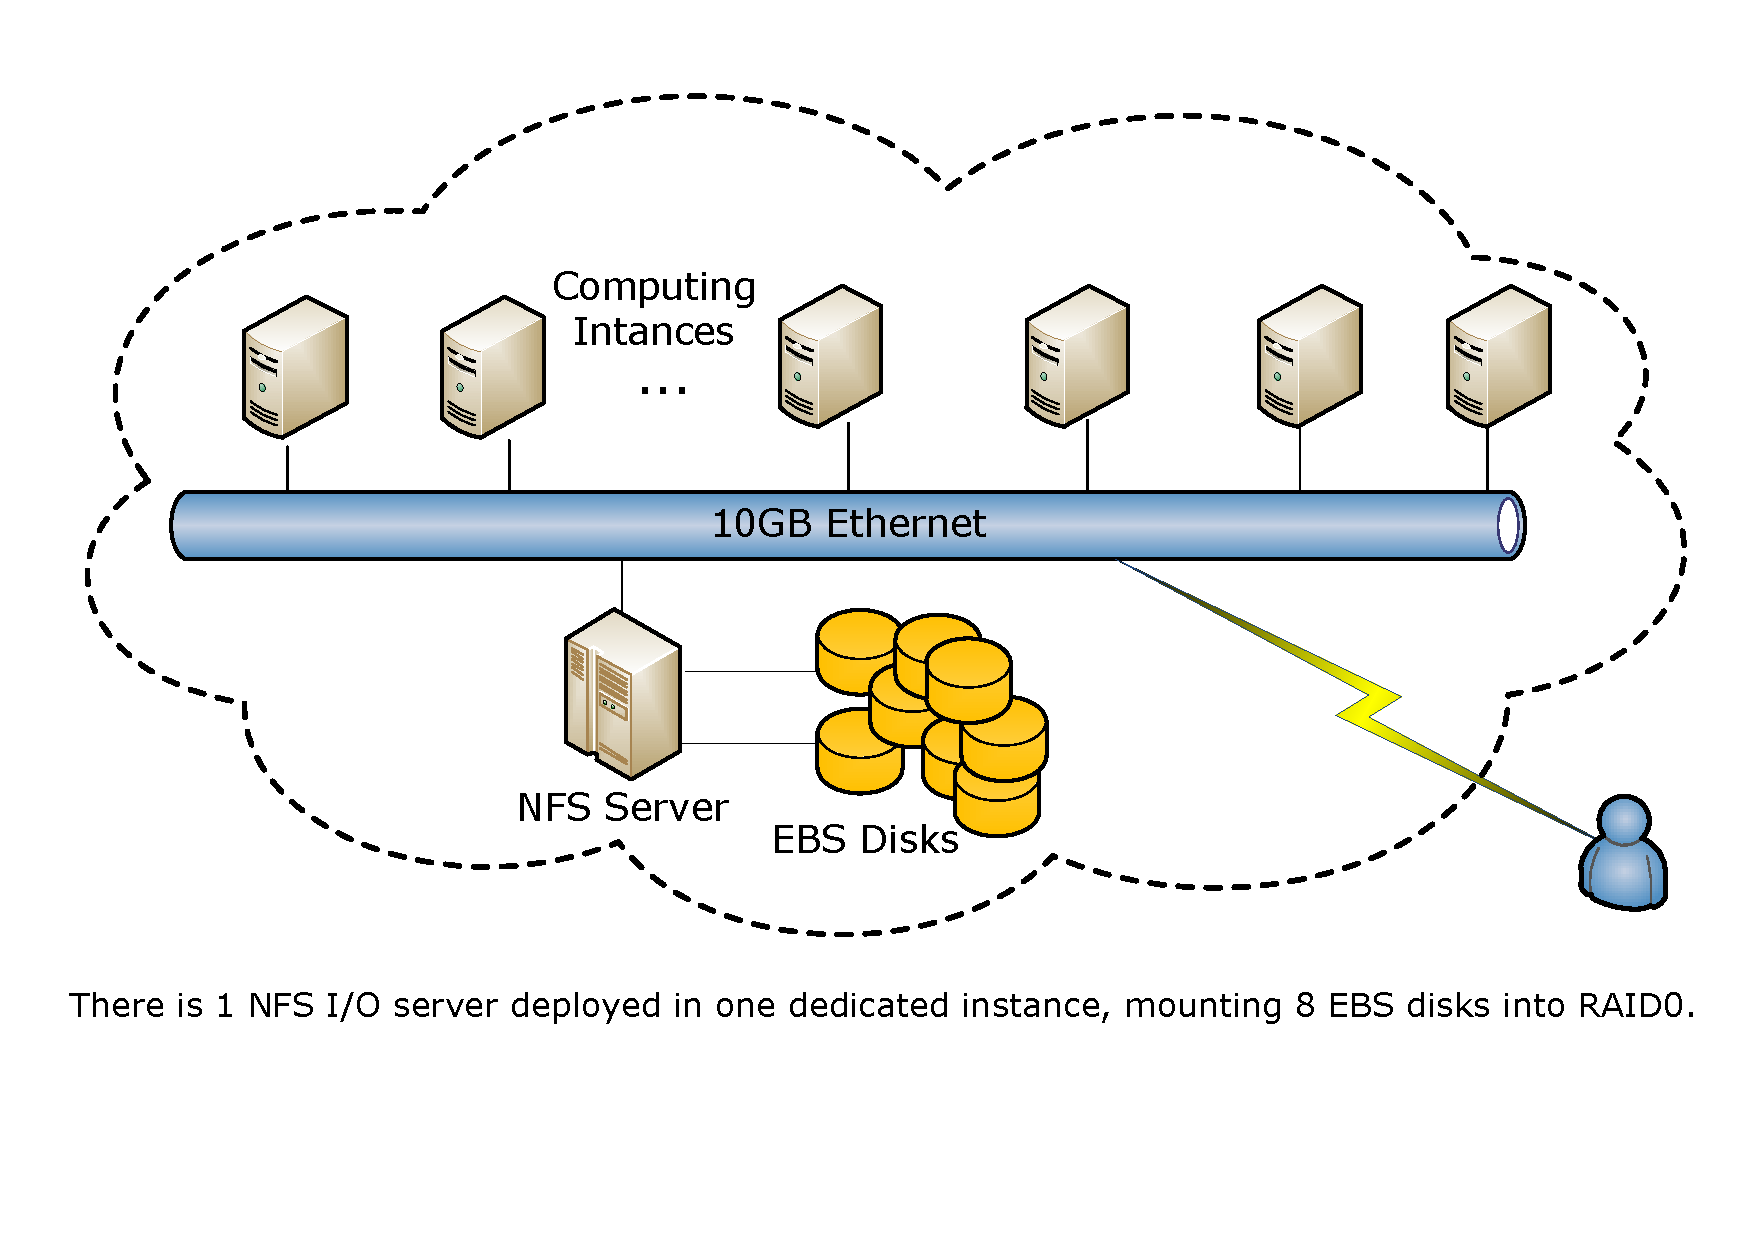
\includegraphics[width=\textwidth]{figures/visio/nfs-ebs.pdf}
    \end{center}
\end{frame}

\begin{frame}{1 Dedicated PVFS I/O server}
    \begin{center}
        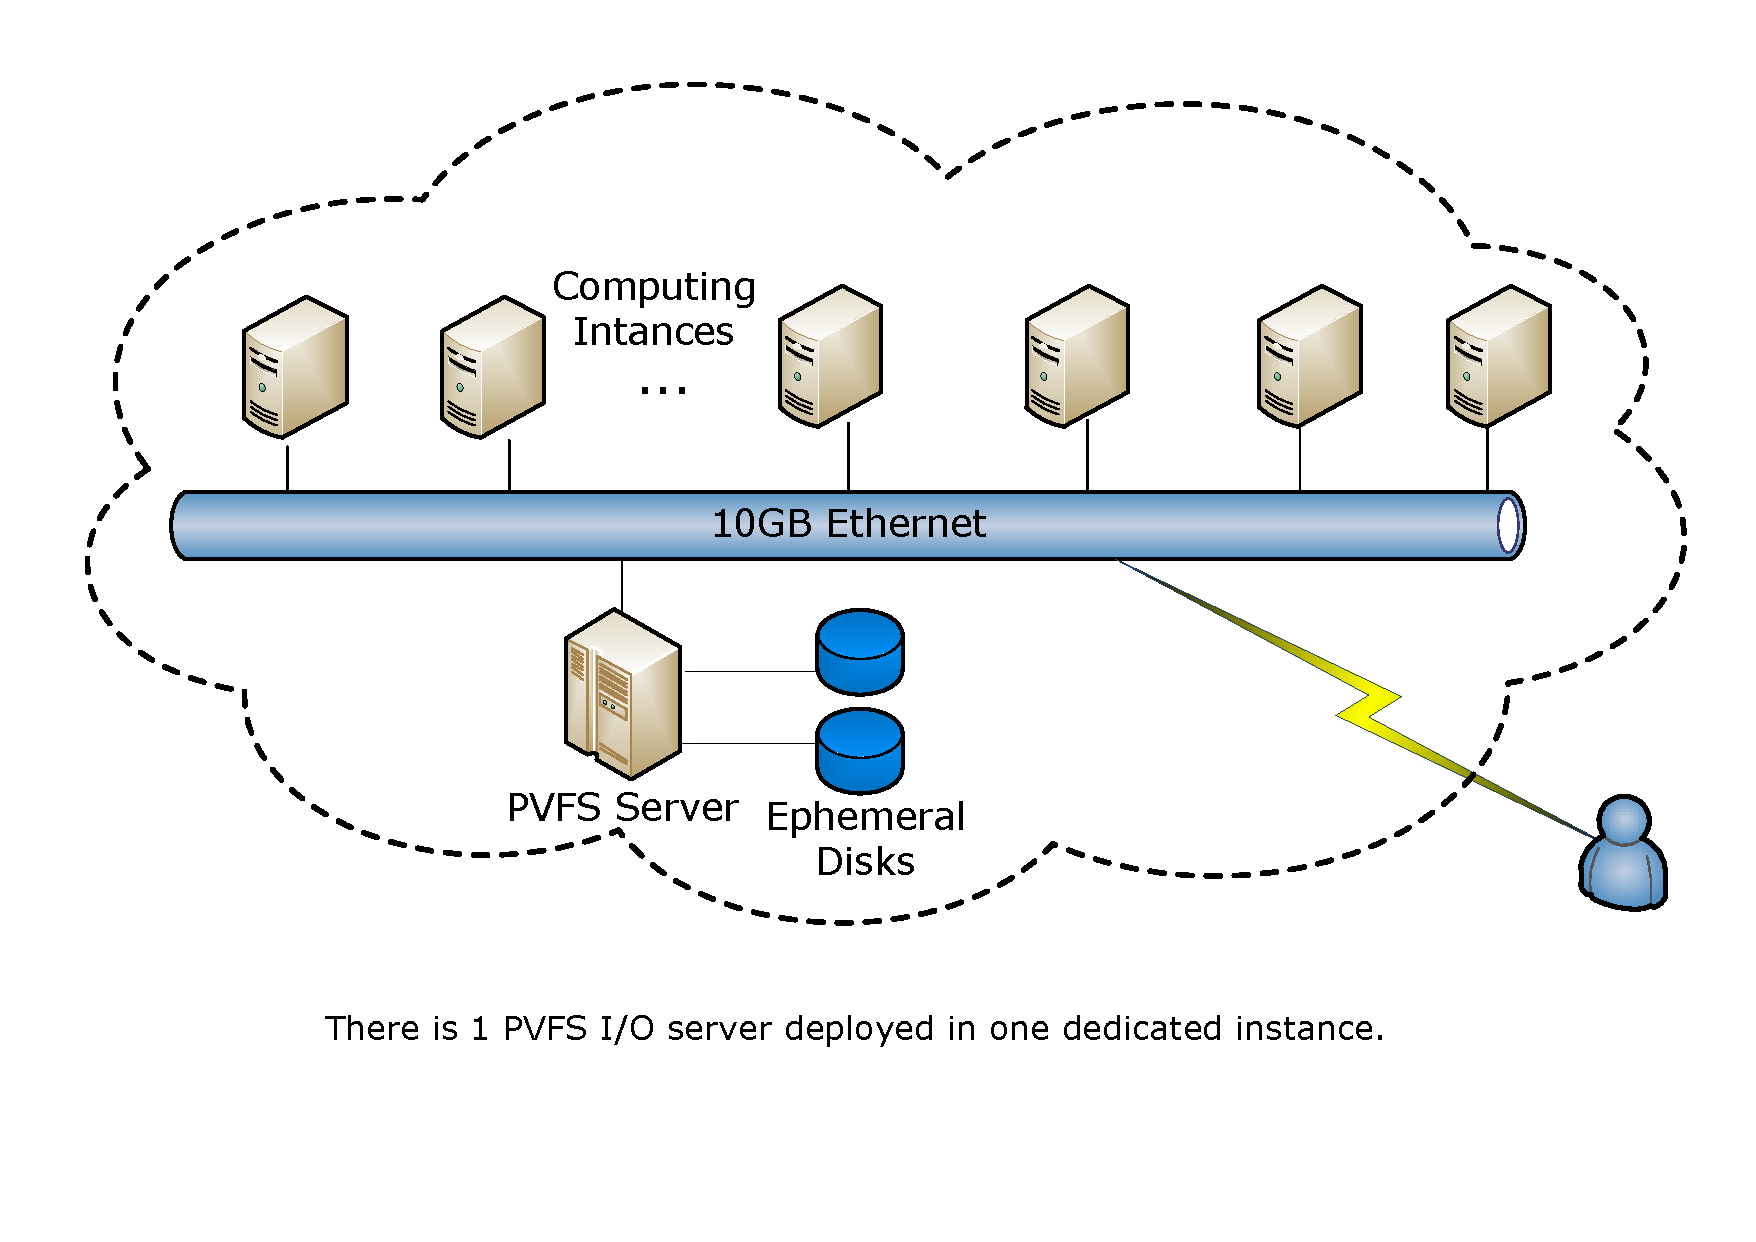
\includegraphics[width=\textwidth]{figures/visio/pvfs-1.pdf}
    \end{center}
\end{frame}

\begin{frame}{2 Dedicated PVFS I/O Servers}
    \begin{center}
        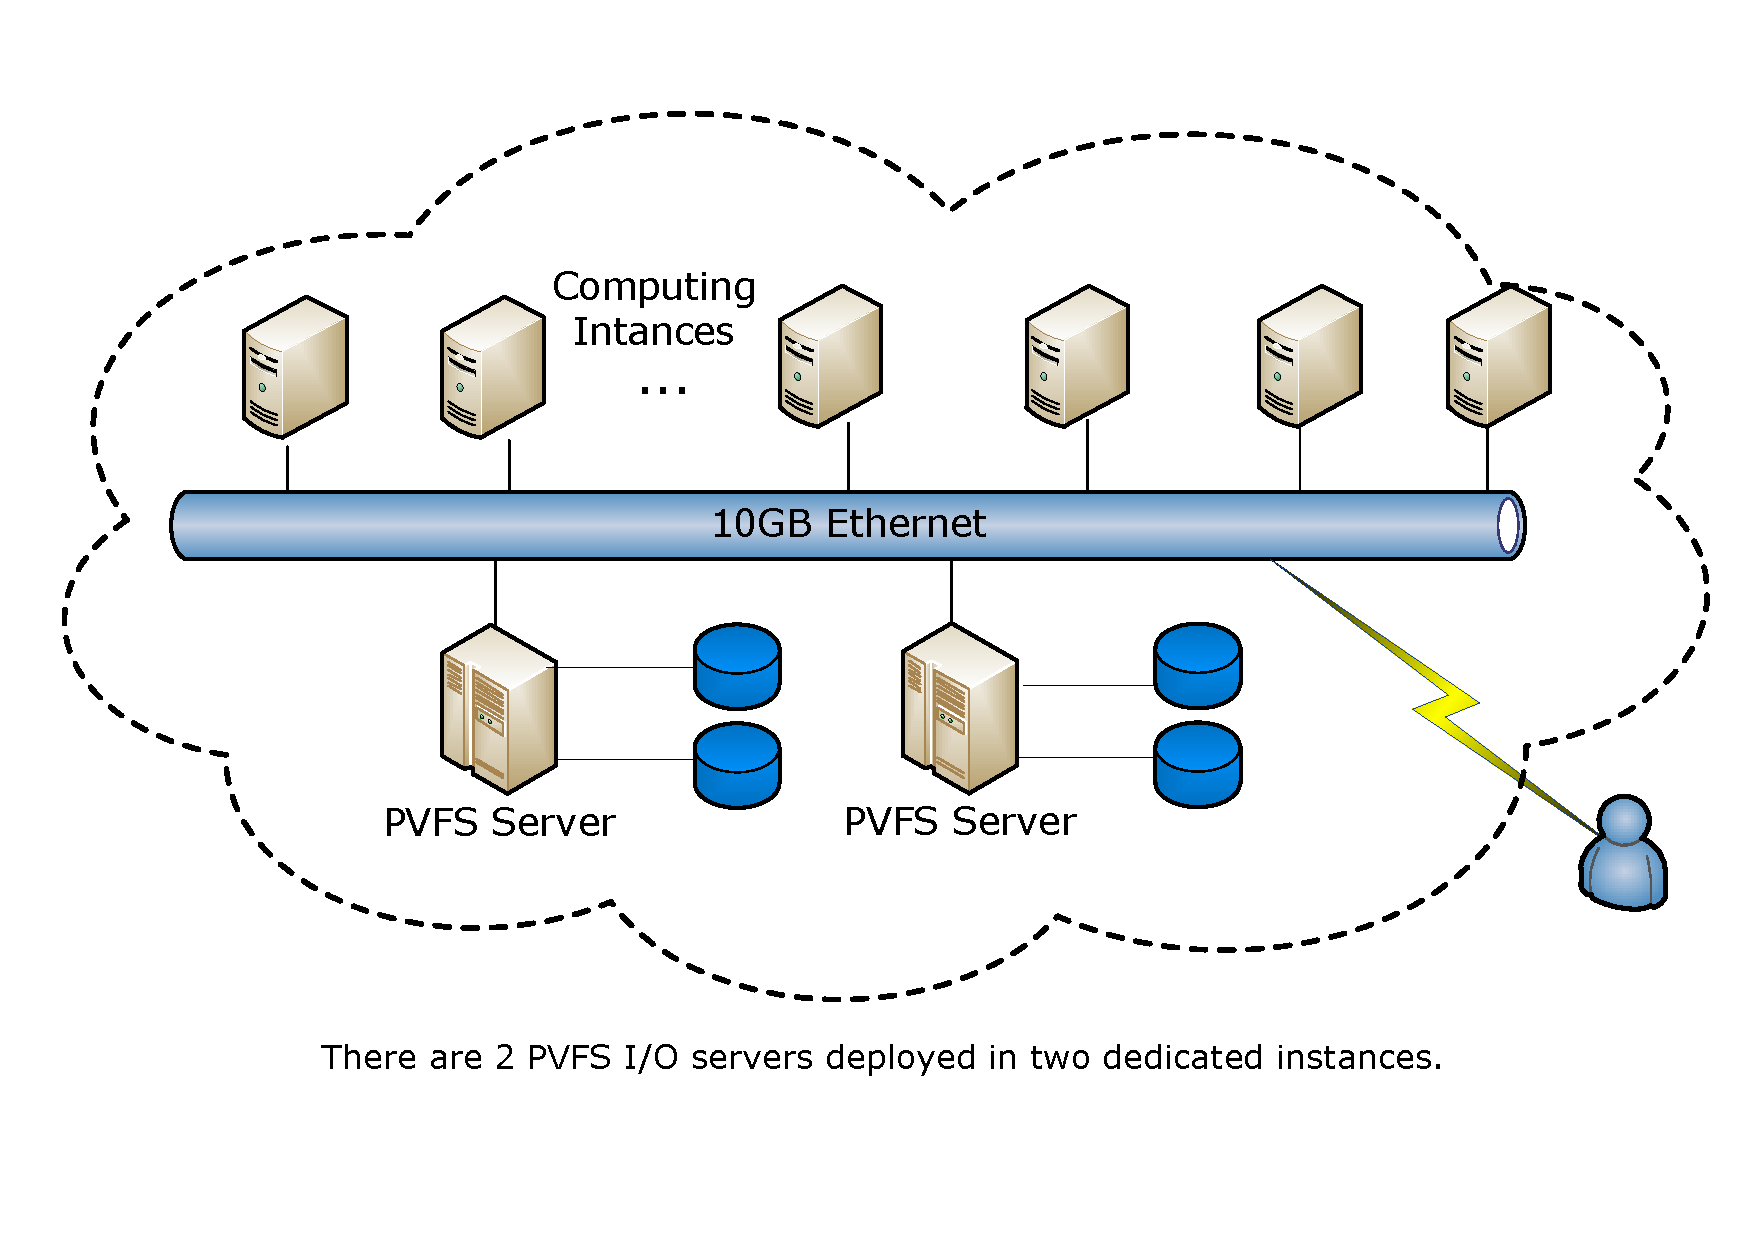
\includegraphics[width=\textwidth]{figures/visio/pvfs-2.pdf}
    \end{center}
\end{frame}

\begin{frame}{4 Dedicated PVFS I/O Servers}
    \begin{center}
        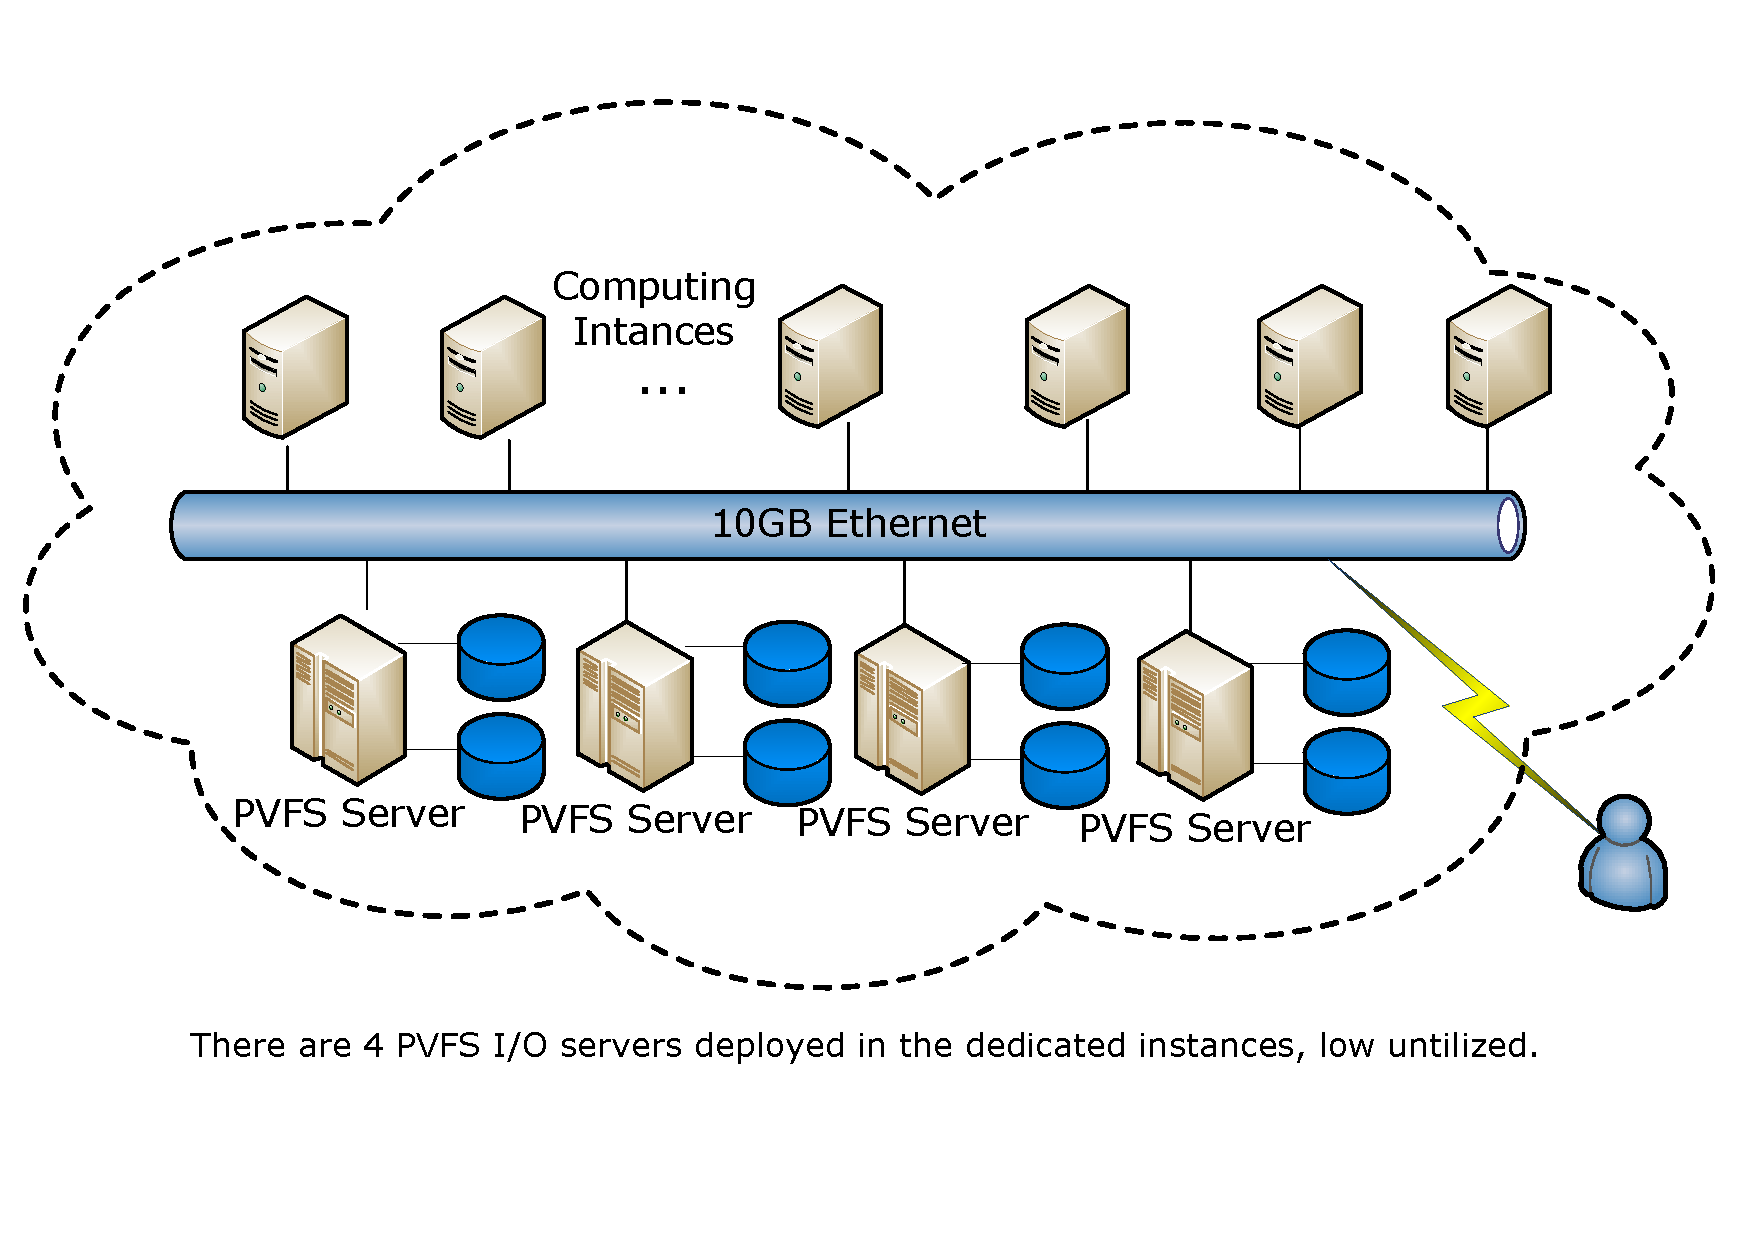
\includegraphics[width=\textwidth]{figures/visio/pvfs-4.pdf}
    \end{center}
\end{frame}

\begin{frame}{4 Part-time PVFS I/O servers}
    \begin{center}
        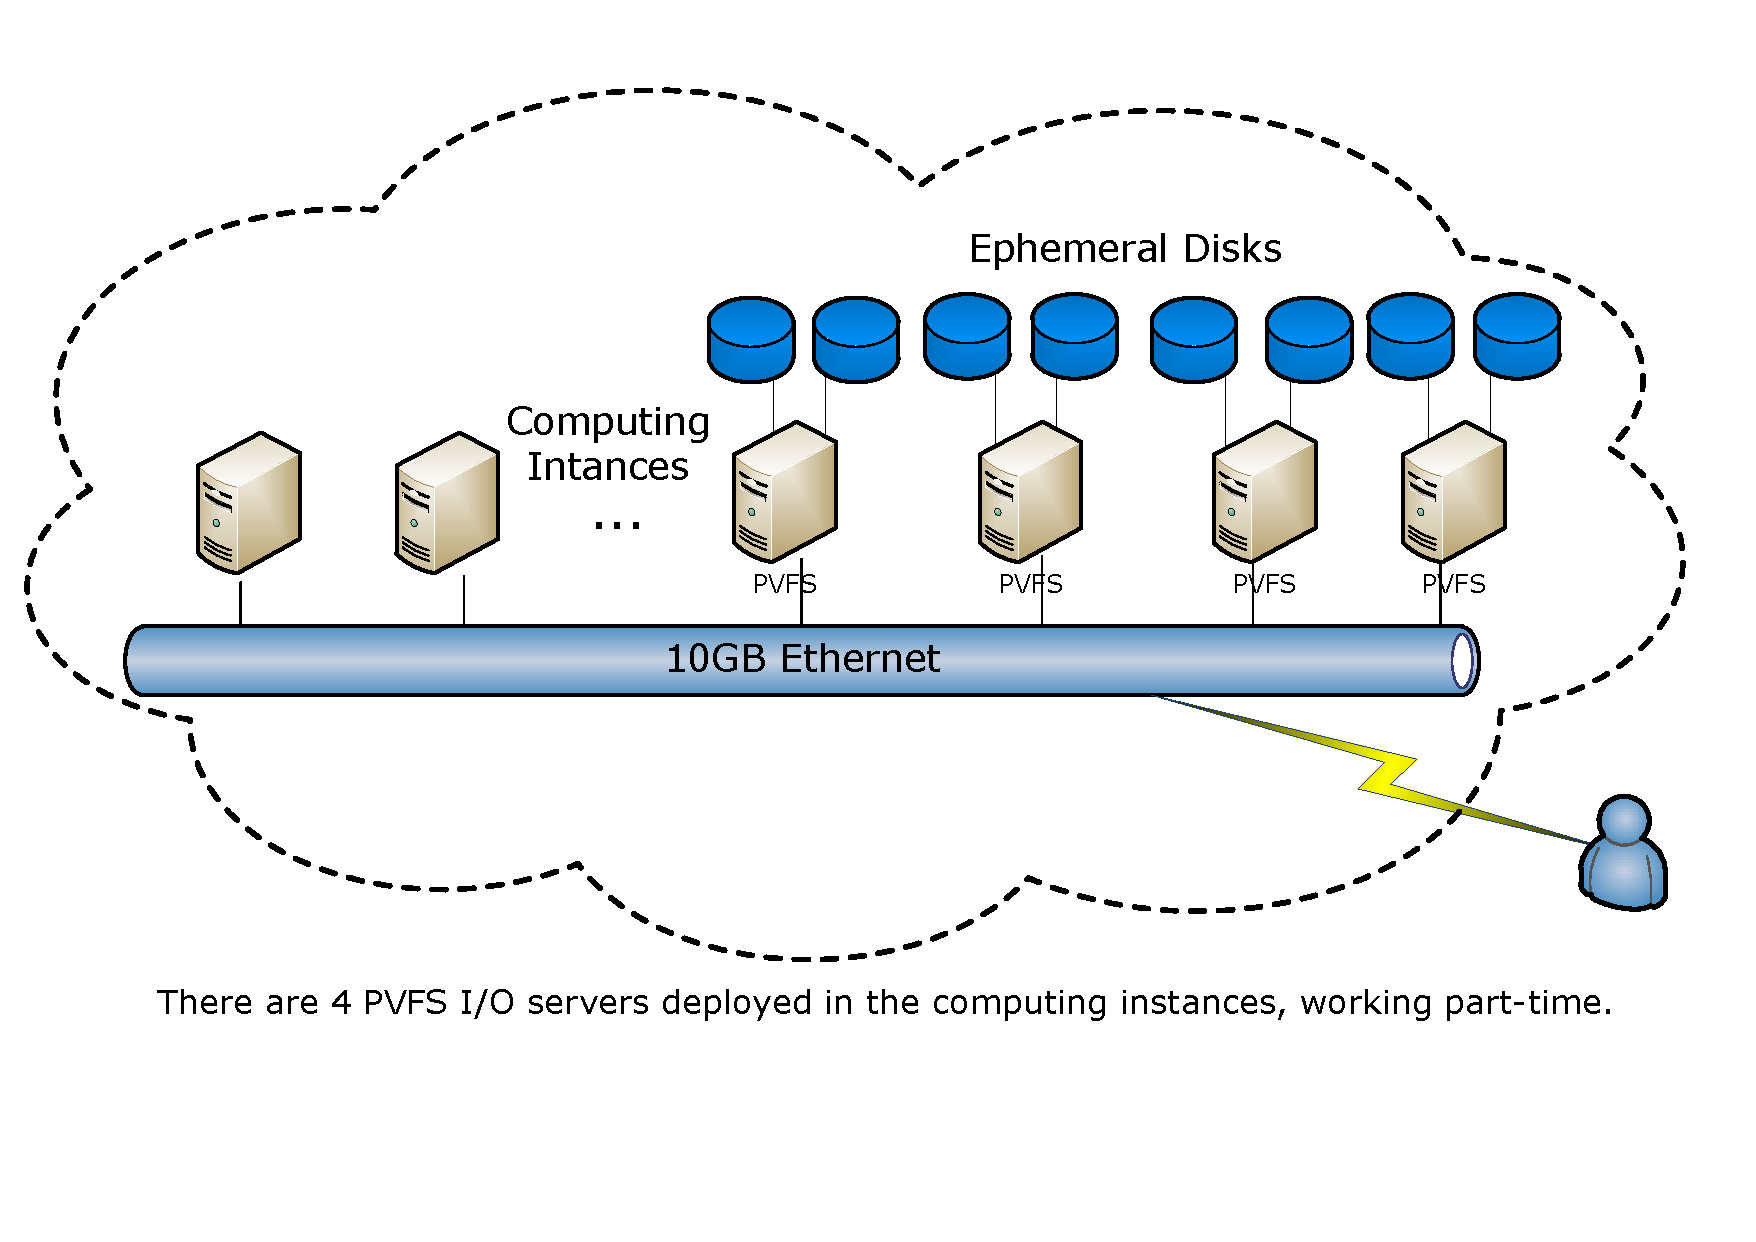
\includegraphics[width=\textwidth]{figures/visio/pvfs-4-parttime.pdf}
    \end{center}
\end{frame}

\begin{frame}{Options: sync mode and device}
    \begin{center}
        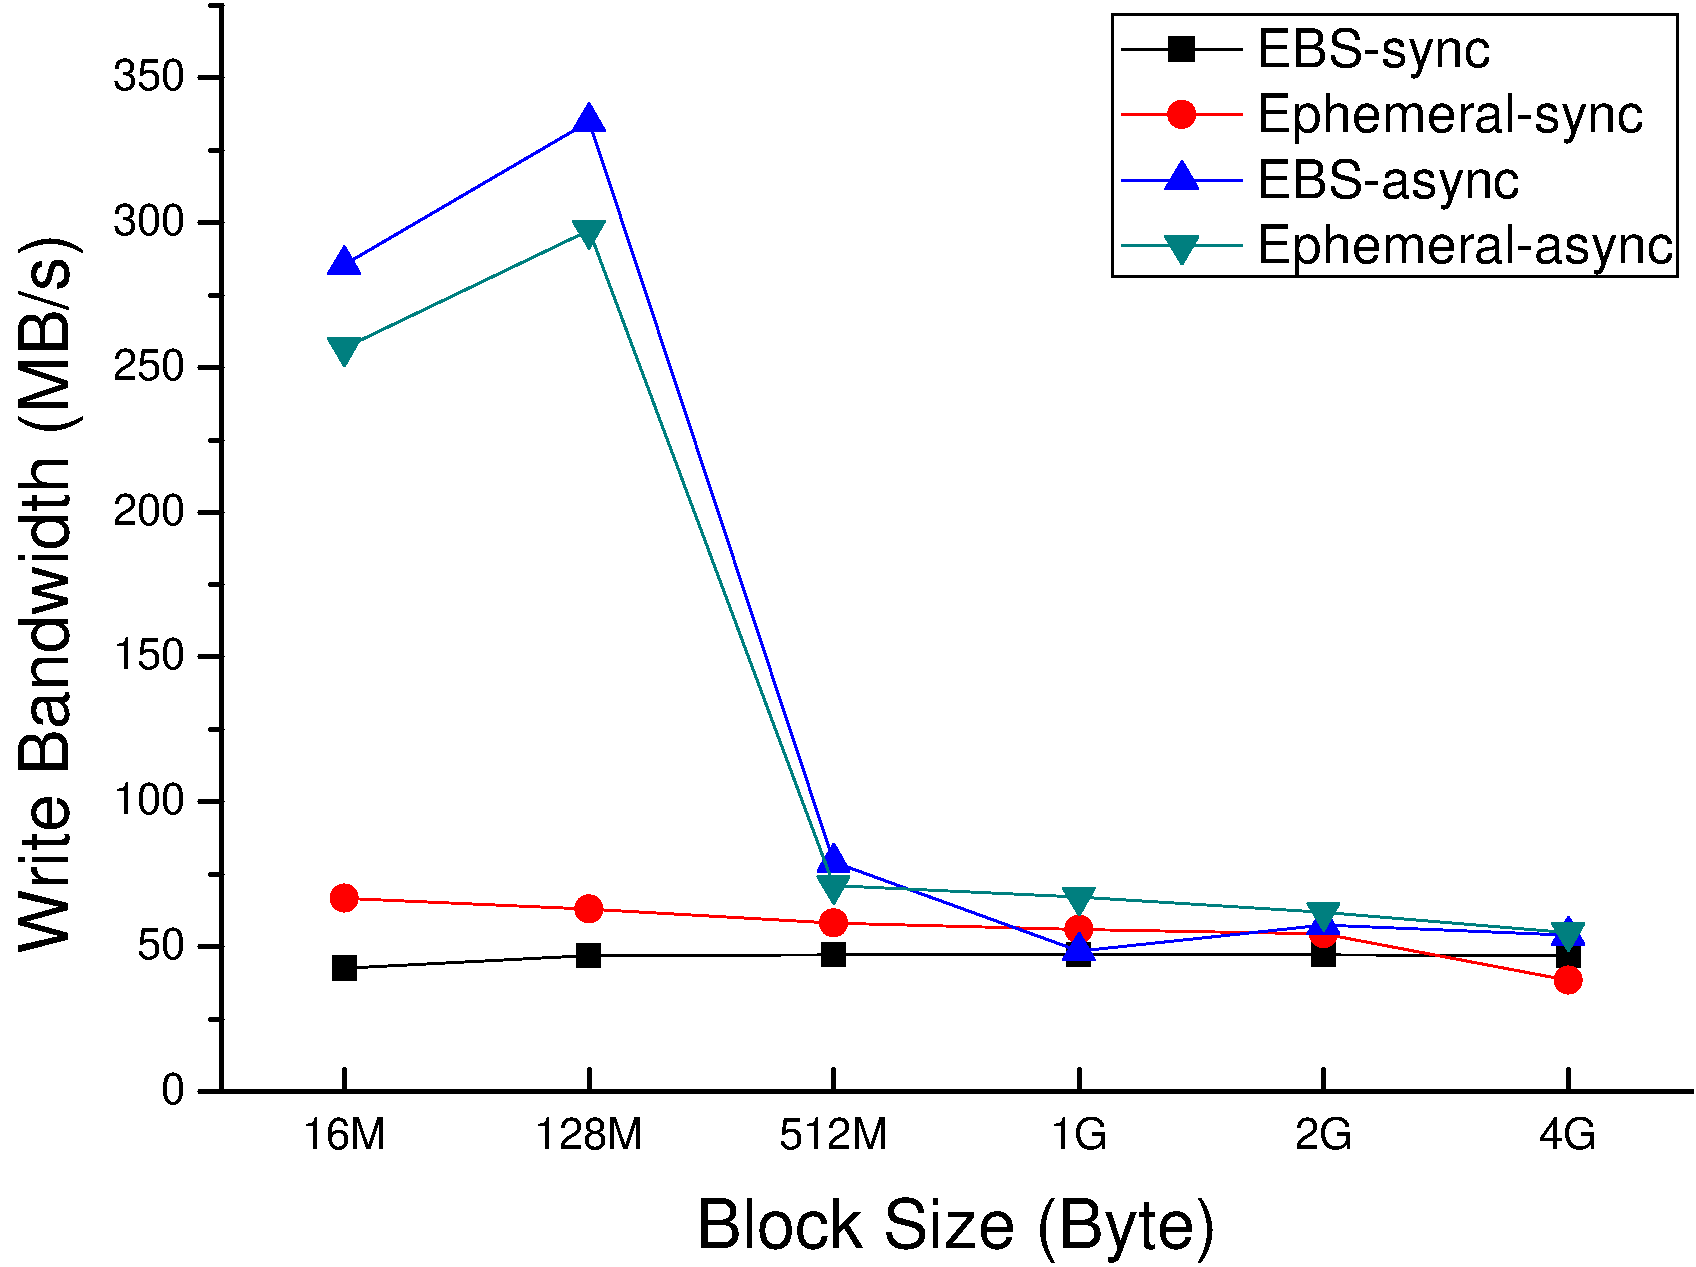
\includegraphics[width=.55\textwidth]{figures/nfs-write}
    \end{center}
    \begin{itemize}
        \item Test by IOR benchmark in 16 processes at 2 nodes.
        \pause
        \item Observations:
            \begin{itemize}
                \item No obvious difference between EBS and ephemeral
                \pause
                \item \texttt{Async} mode prefers small block sizes
            \end{itemize}
    \end{itemize}
\end{frame}

\begin{frame}{NFS Write Bandwidth}
    \begin{center}
        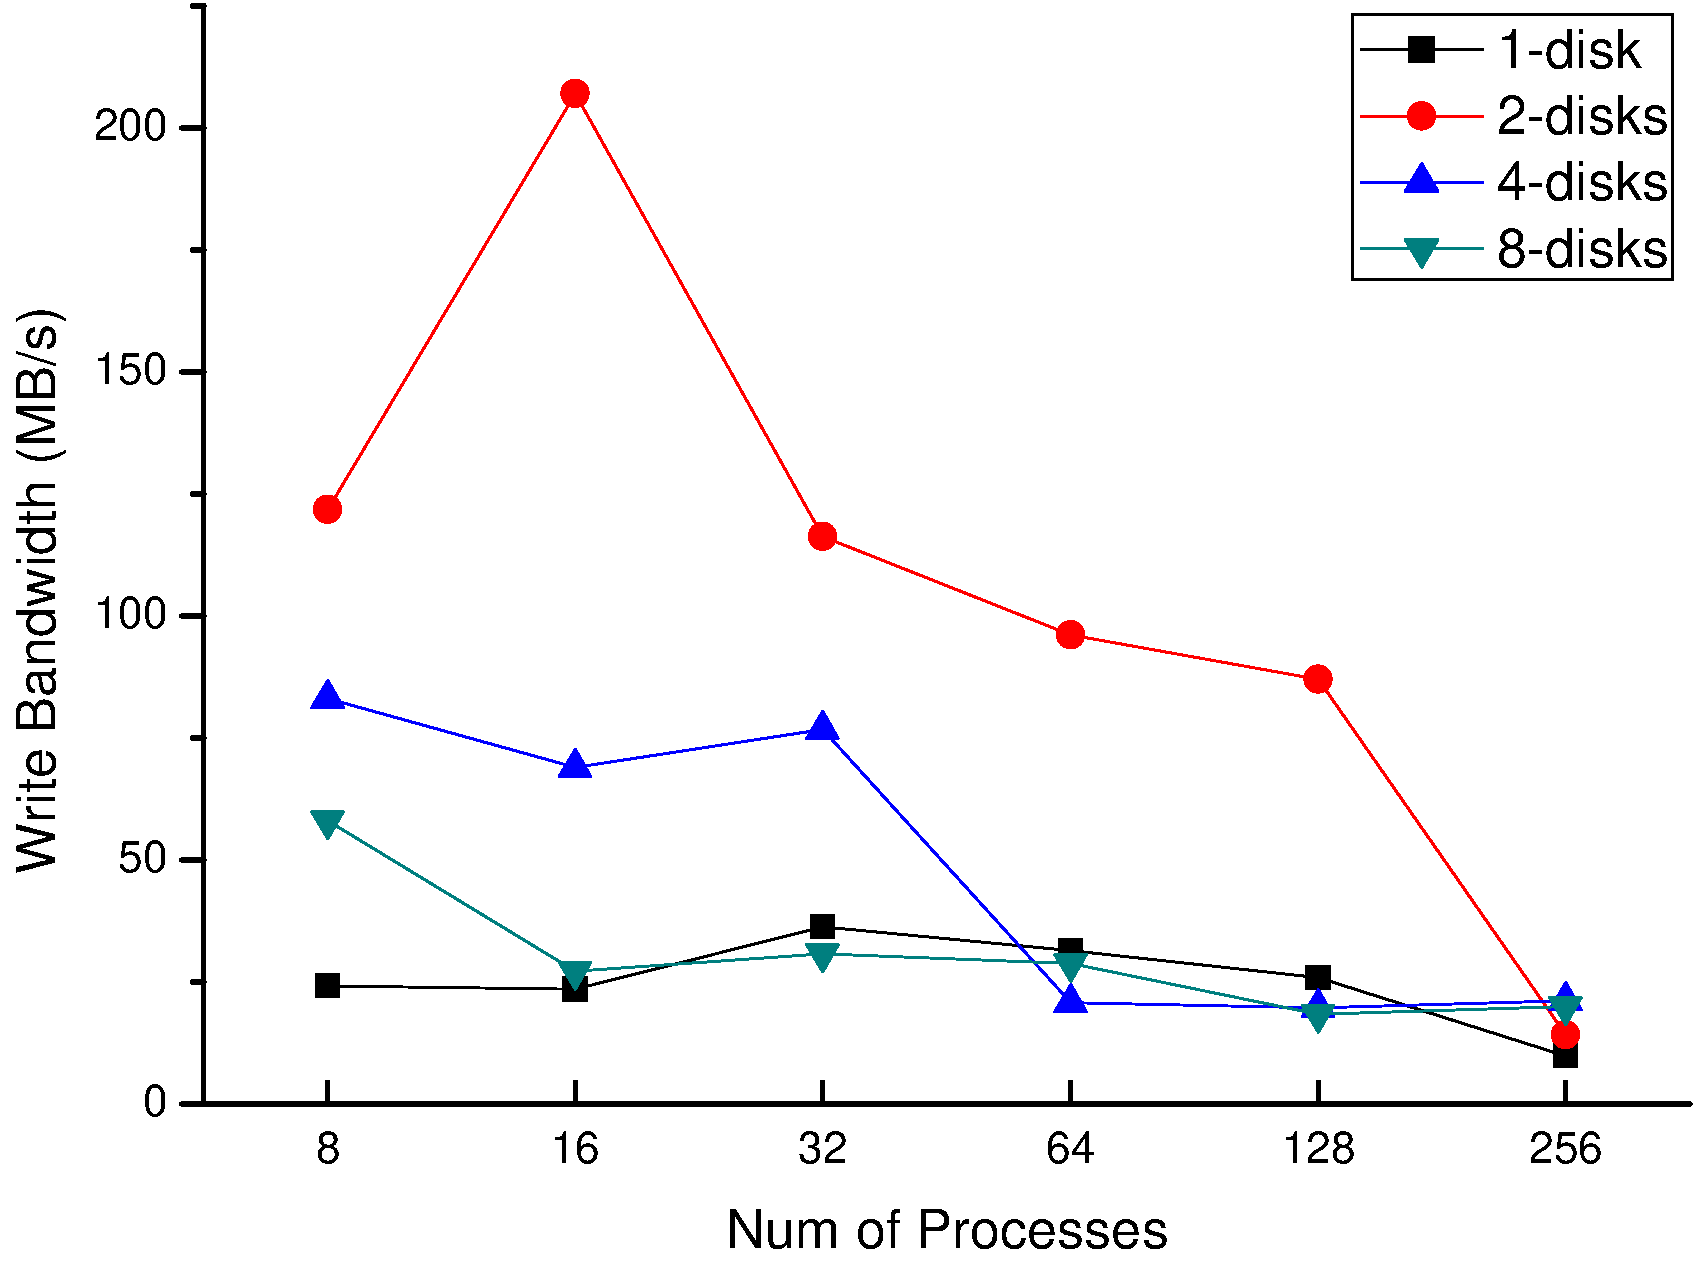
\includegraphics[width=.55\textwidth]{figures/nfs-raid0-write}
    \end{center}
    \begin{itemize}
        \item Combining 1,2,4,8 EBS disks into a software RAID0
        \pause
        \item The RAID0 doesn't scale well\\
            - possibly because of the virtualized layer
    \end{itemize}
\end{frame}

%%%%%%%%%%%%%%%%%%%%%%% Preliminary Applications Results %%%%%%%%%%%%%%%%%%%%%
\section{Preliminary Applications Results}
\begin{frame}{Outline}
    \tableofcontents[current]
\end{frame}

\begin{frame}{BTIO: CLASS=\texttt{C}, SUBTYPE=\texttt{full}}
    \begin{center}
        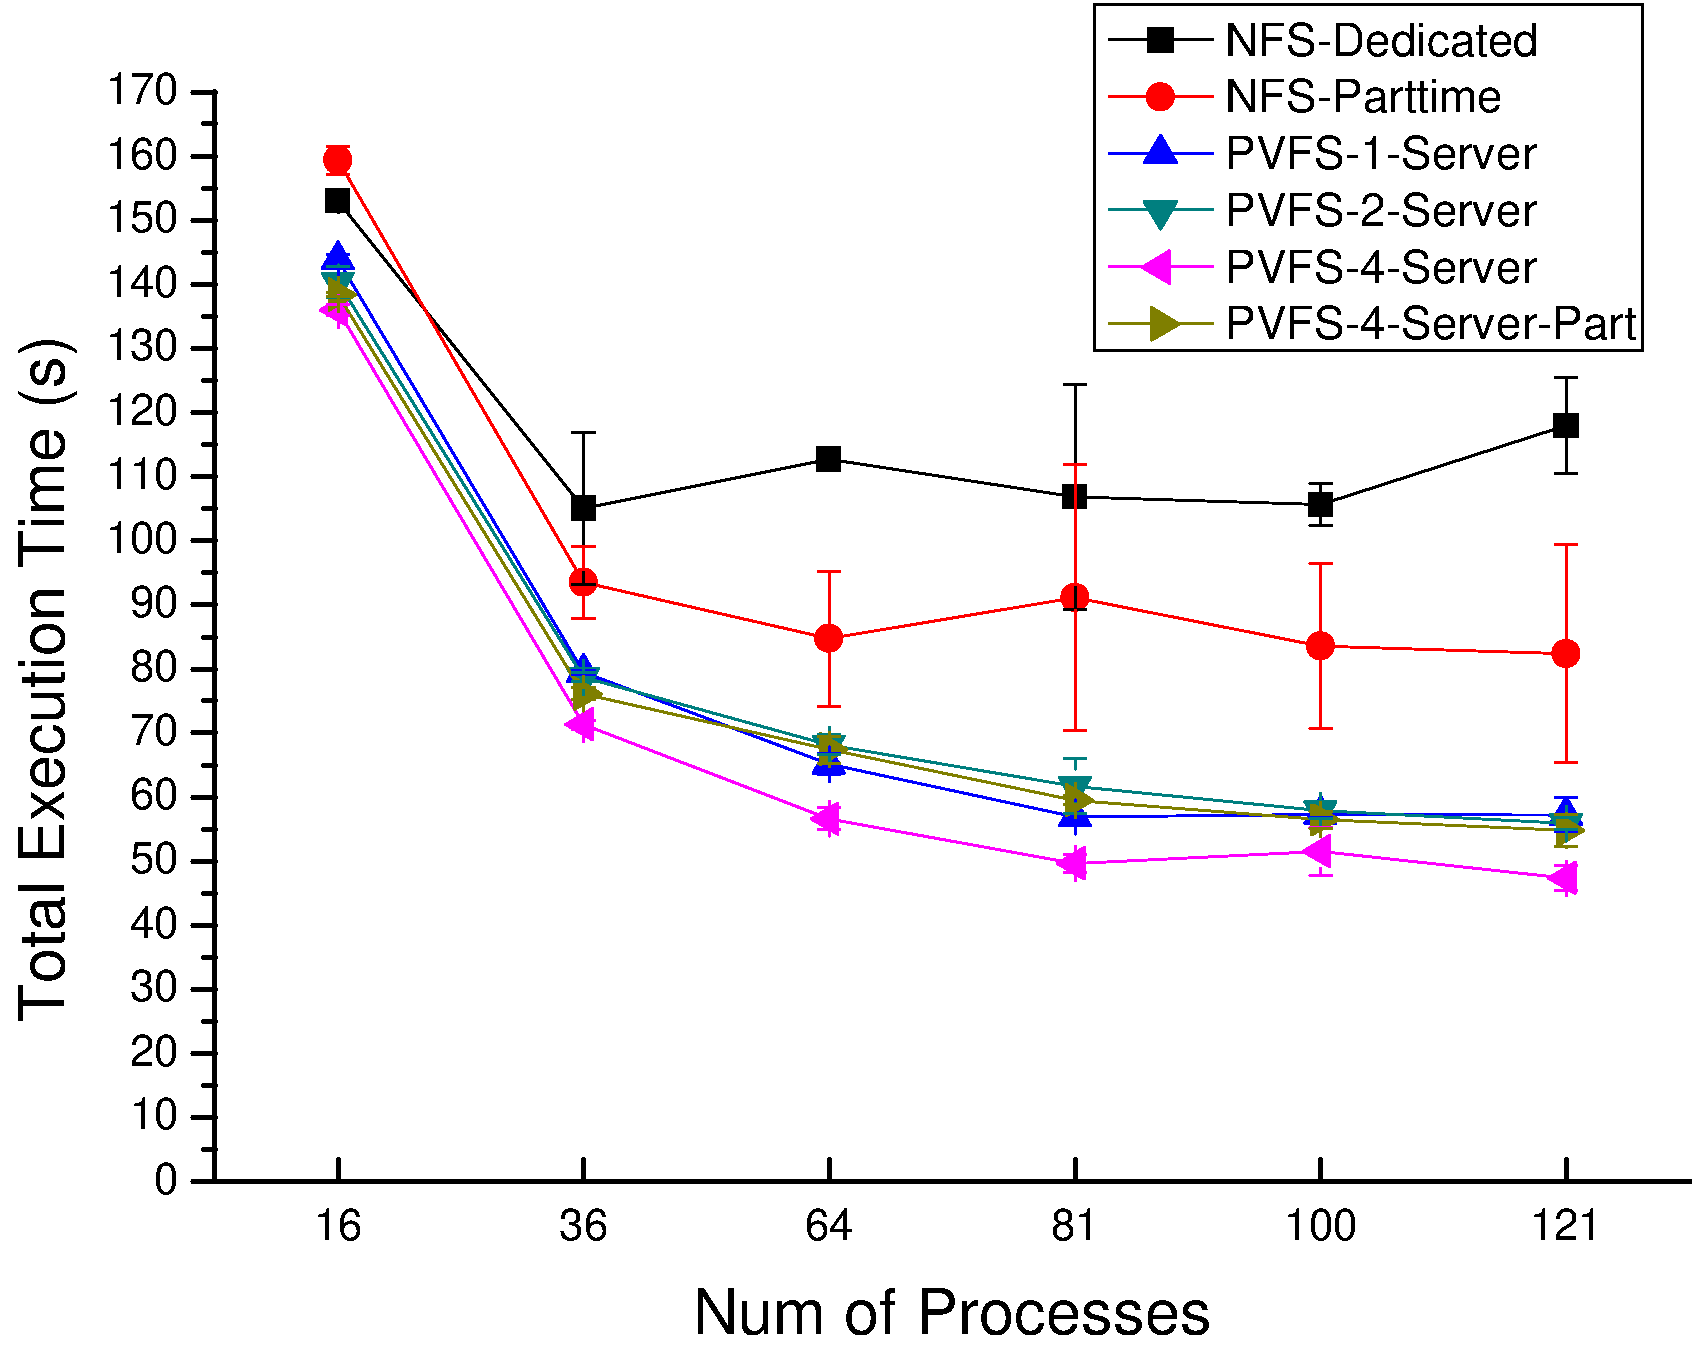
\includegraphics[width=.55\textwidth]{figures/T-time}
    \end{center}
    \pause
    \begin{itemize}
        \item PVFS outperforms NFS configurations all the time
        \pause
        \item PVFS scales up by adding more I/O servers
        \pause
        \item Parttime I/O servers provide pretty good performance
    \end{itemize}
\end{frame}

\begin{frame}{BTIO: Total Cost Analysis}
    \begin{exampleblock}{Cost calculation}
        $Cost (\$) = Num_{computing~instances} * Run\_time * 1.6 / 3600 $
    \end{exampleblock}
    \begin{center}
        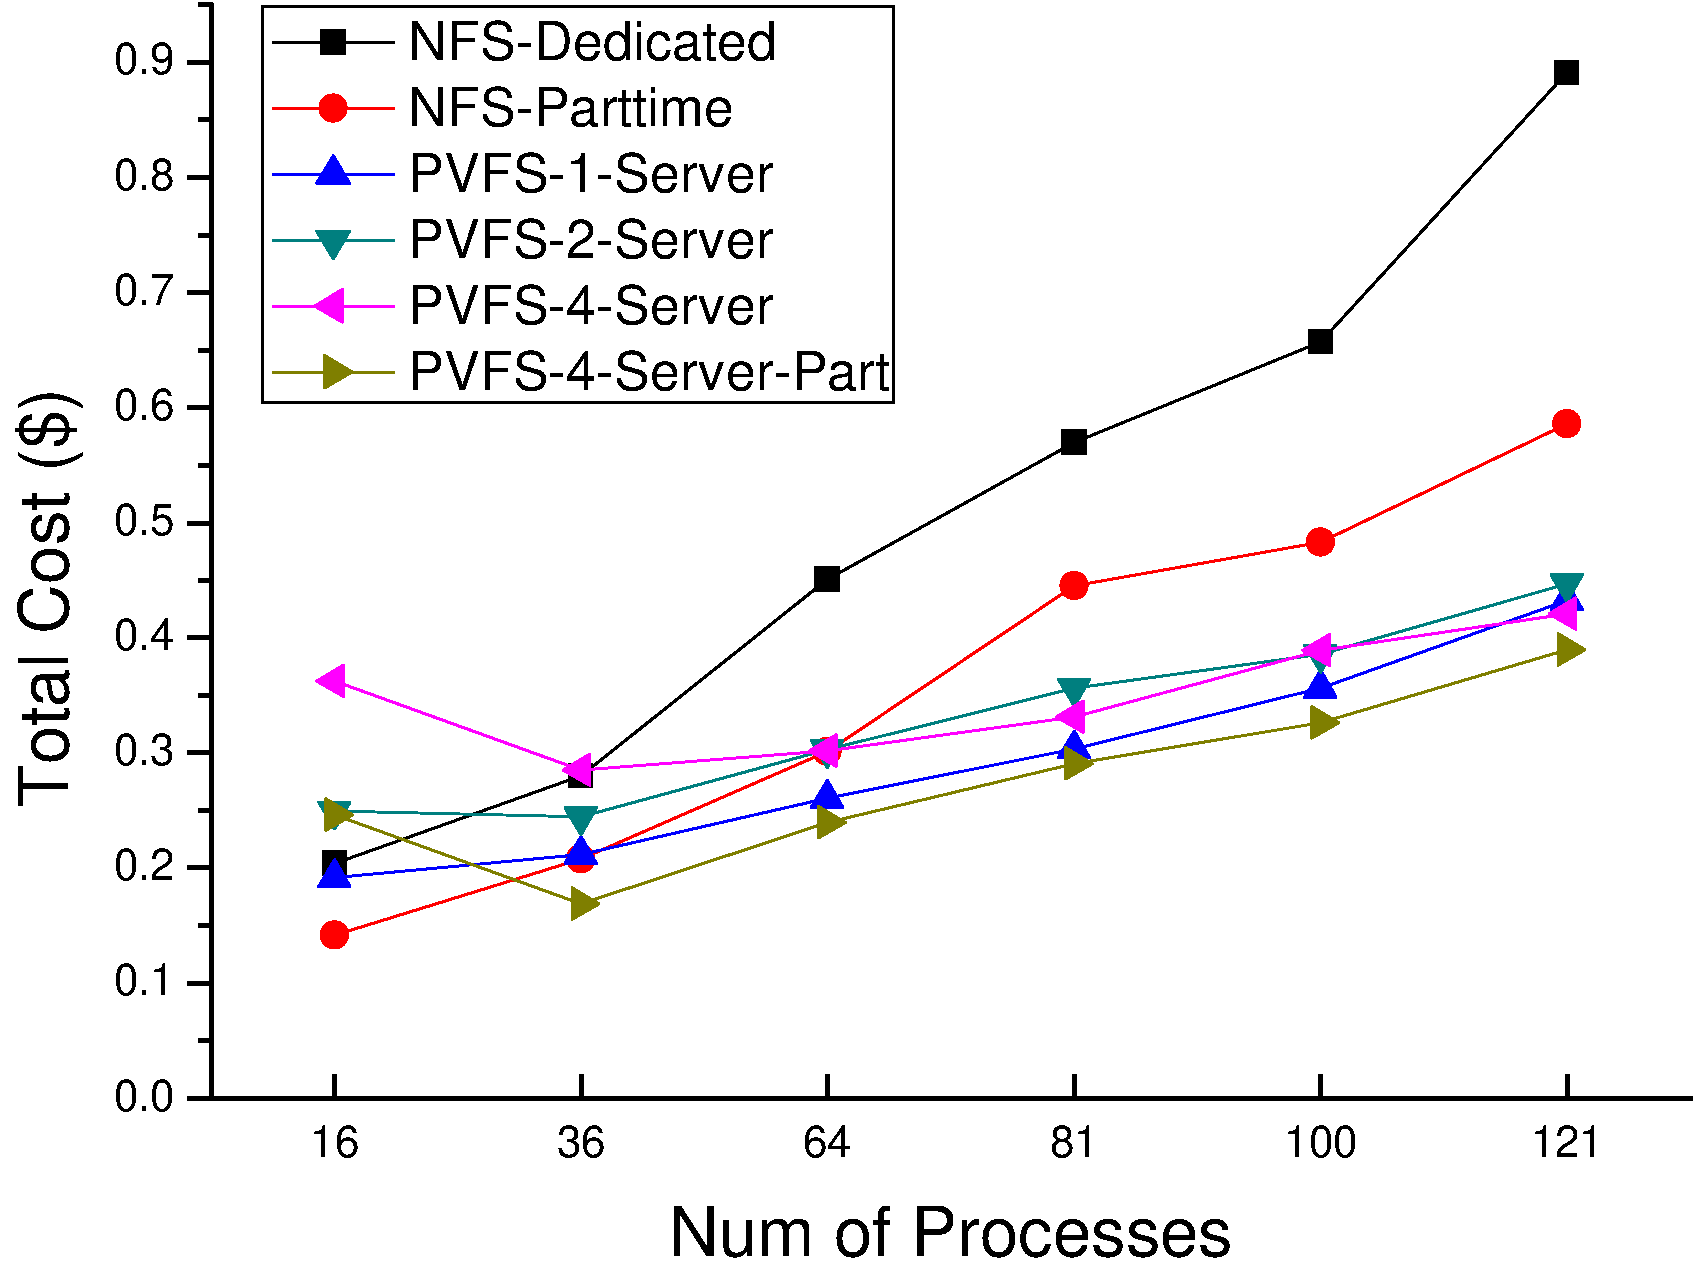
\includegraphics[width=.6\textwidth]{figures/T-cost}
    \end{center}
\end{frame}

\begin{frame}{POP: Parallel Ocean Program}
    \begin{itemize}
        \item Process 0 carries out all I/O tasks via POSIX interface, which
            is very different from BTIO
        \item POP does not scale on EC2, due to its heavy communication with
            small messages
    \end{itemize}
    \begin{center}
        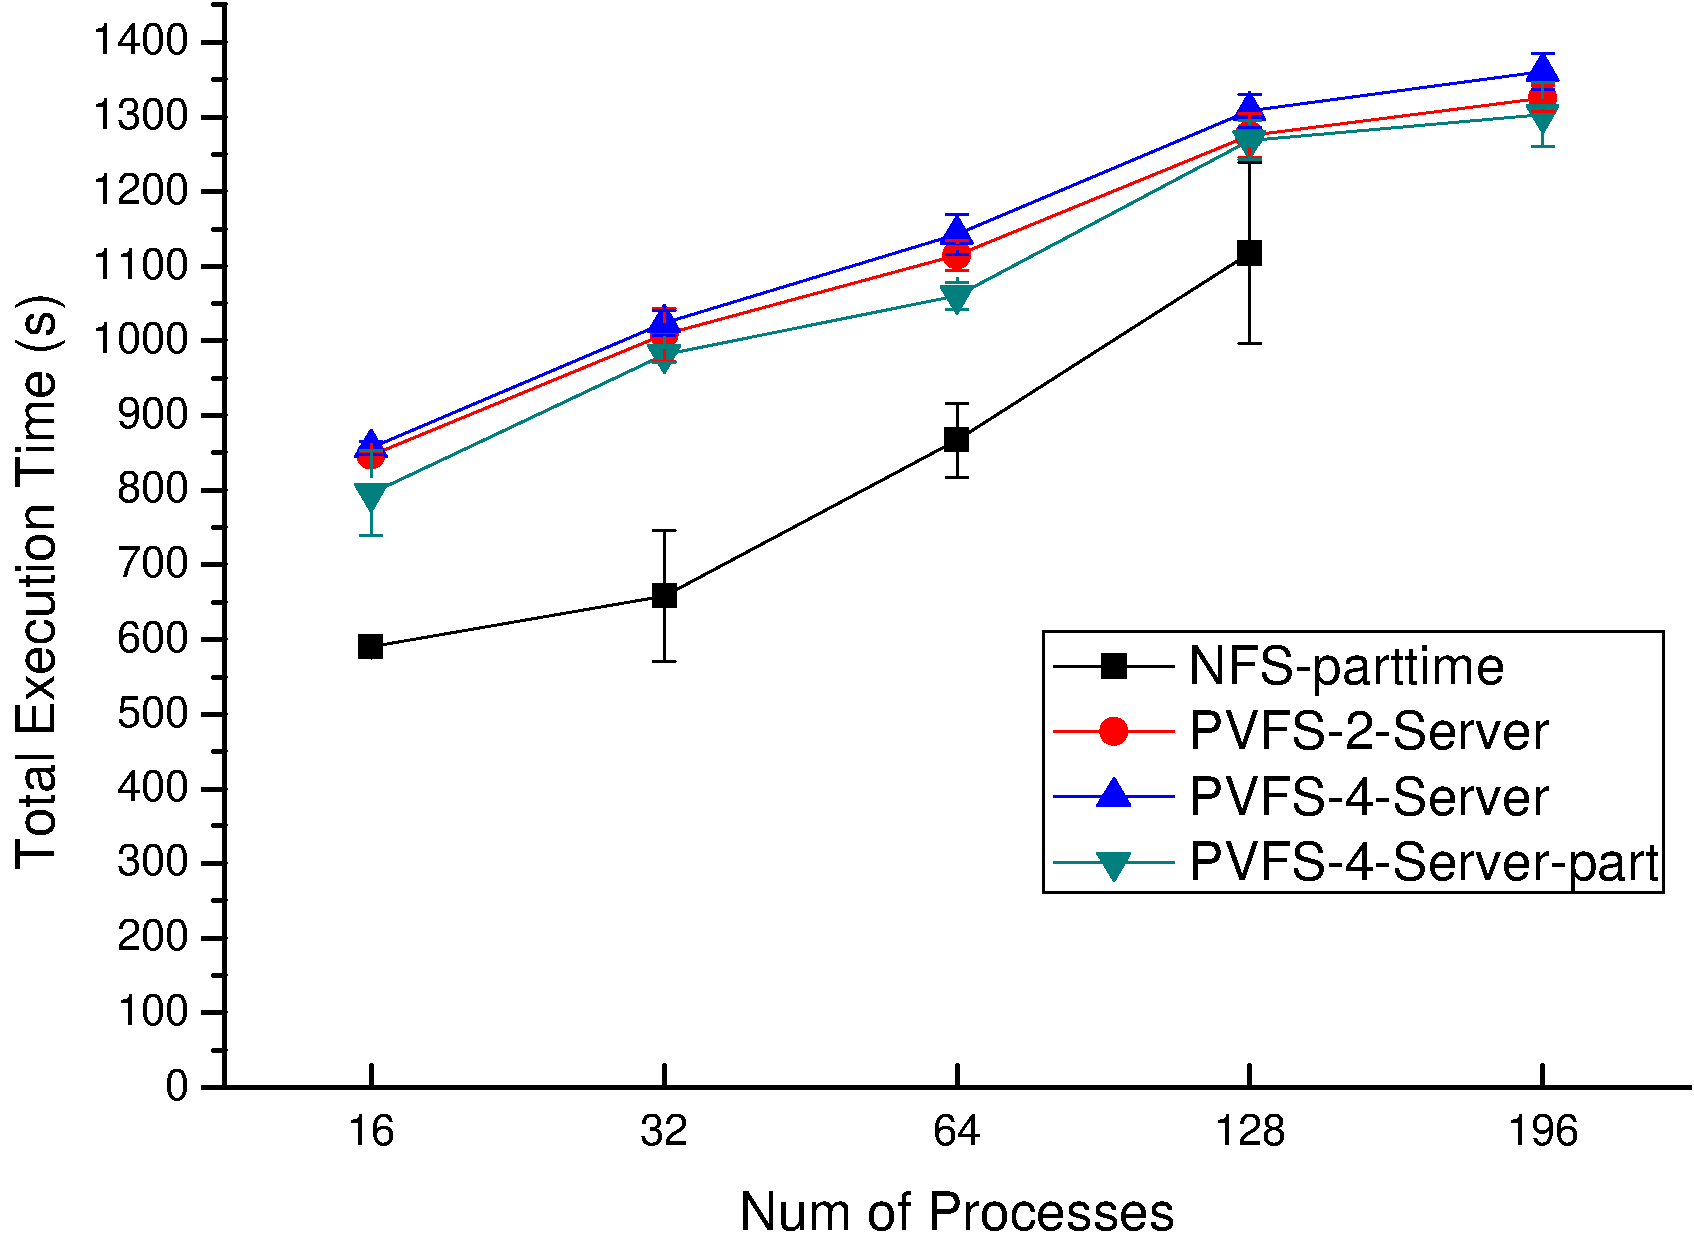
\includegraphics[width=.5\textwidth]{figures/pop}
    \end{center}
\end{frame}

%%%%%%%%%%%%%%%%%%%%%%% Discussion %%%%%%%%%%%%%%%%%%%%%%
\section{Conclusion}
\begin{frame}{Outline}
    \tableofcontents[current]
\end{frame}

\begin{frame}{Future Work}
    \begin{block}{The Problem}
        Configure the I/O system for a HPC app \emph{automatically}
    \end{block}
    \begin{center}
        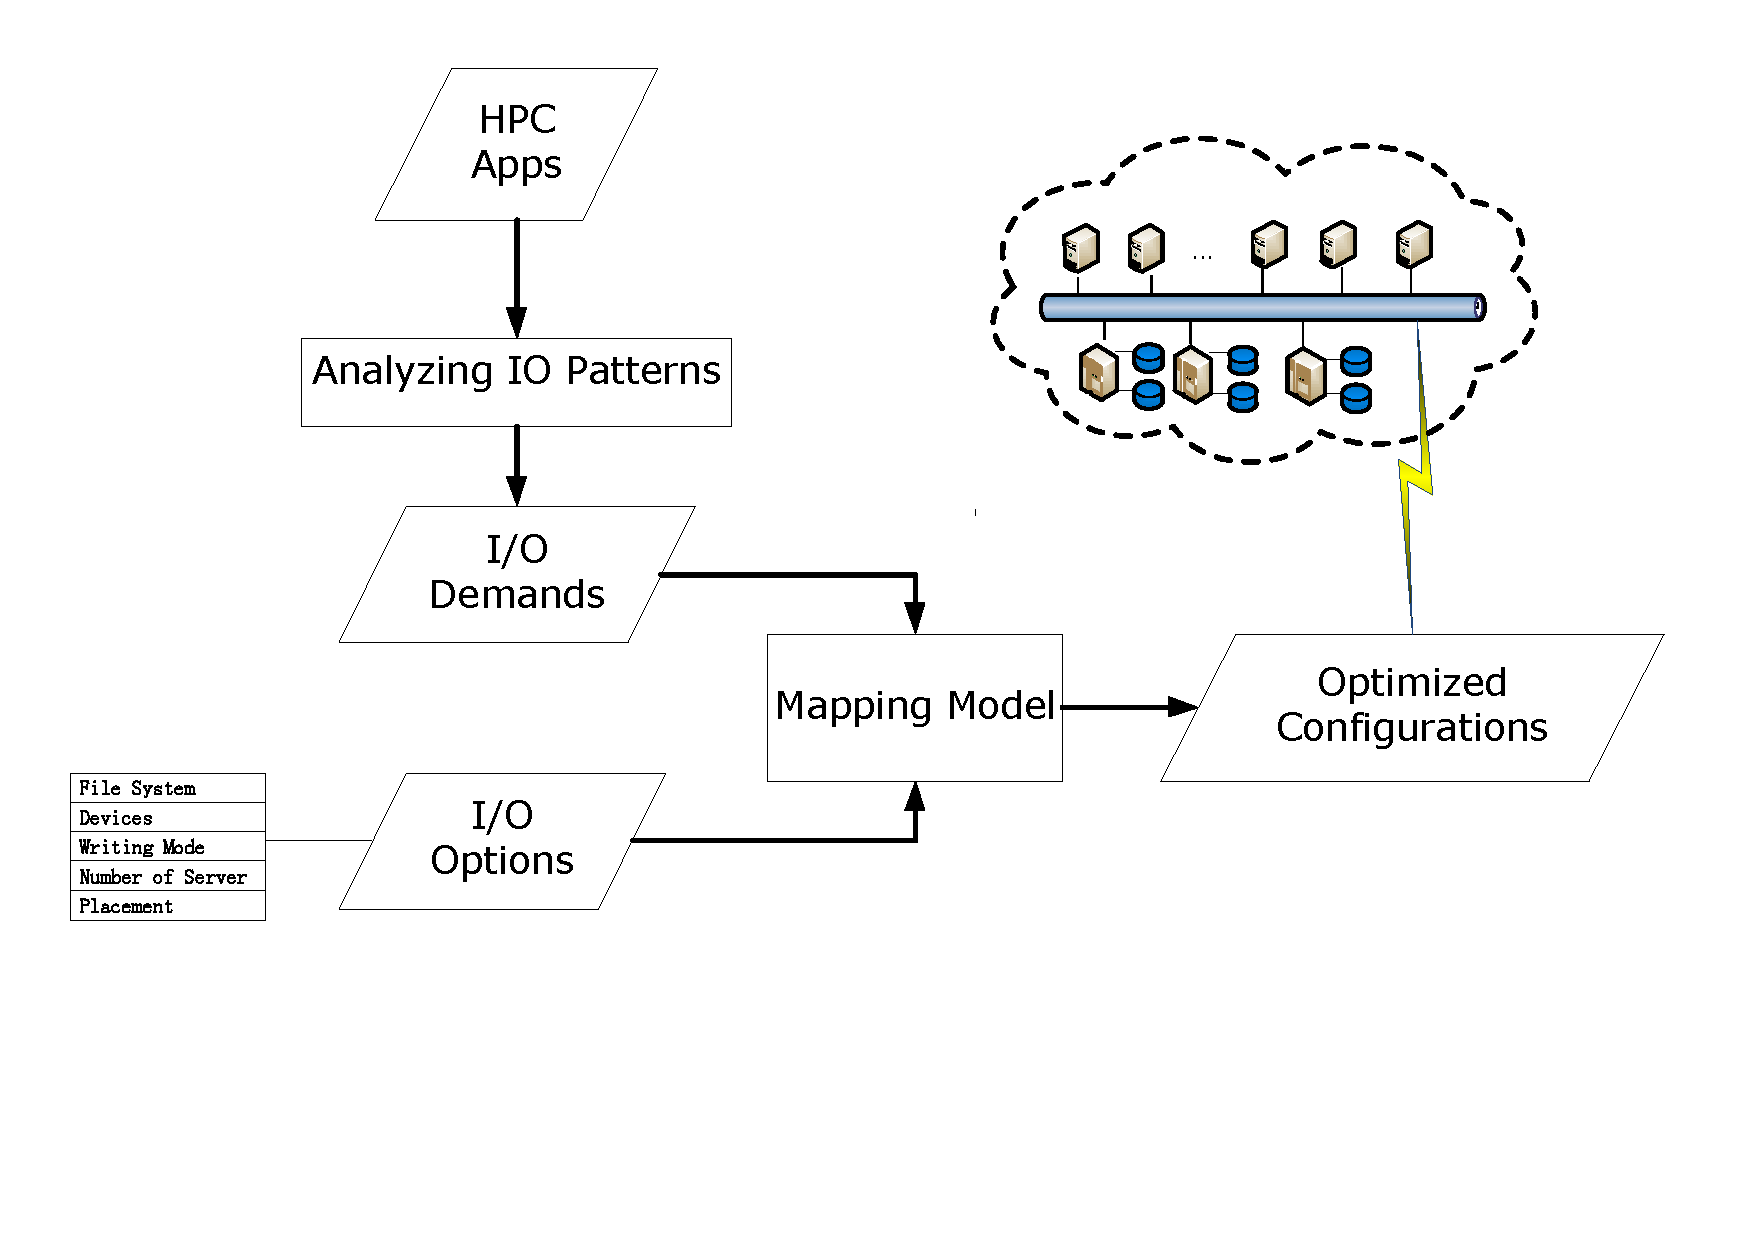
\includegraphics[width=.9\textwidth]{figures/visio/future.pdf}
    \end{center}
\end{frame}

\begin{frame}{Conclusion}
    \begin{itemize}
        \item Cloud enables users to build per-application I/O systems
        \item Our preliminary results hint that
            \begin{itemize}
                \item HPC app behaves differently with different I/O system
                    configurations in cloud
                \item Configuration per app depends on its I/O access pattern
                    and concurrency
            \end{itemize}
        \item Tradeoff: cost vs. efficiency
        \pause
        \begin{center}\shadowbox{\structure{\huge Thank you!}}\end{center}
    \end{itemize}
\end{frame}

\end{document}
